%--------------------导言--------------------%
\documentclass{report}
\usepackage{xcolor}
\usepackage{fancyhdr}%导入fancyhdr包
\usepackage{ctex}%导入ctex包
\usepackage{graphicx}
\pagenumbering{Roman}%设置页码格式,大写字母标页
\pagestyle{fancy}
\fancyhead[L]{}
\fancyhead[R]{\textcolor{gray}{课程实验}}
\fancyhead[L]{\textcolor{gray}{《深度学习》}}
\fancyfoot[L]{\textcolor{gray}{北京理工大学}}
\fancyfoot[C]{\thepage}
\fancyfoot[R]{\textcolor{gray}{计算机学院}}
\renewcommand{\headrulewidth}{0.4pt}%分隔线宽度4磅
\renewcommand{\footrulewidth}{0.4pt}
\usepackage{setspace}
\setstretch{1.2}

%\title{2021-2022学年第2学期\\《深度学习》\\课程实验报告\\ \quad \\ \textbf{实验一:基于全连接网络的手写数字识别}}
%\author{姓名:肖良寿 \qquad 学号:1120200563}
%\date{\today}

%--------------------正文--------------------%
\begin{document}
	\begin{titlepage}
		\begin{center}
			\setstretch{1.5} % 设置行间距为1.5倍
			{\LARGE \textbf{2021-2022学年第2学期\\《深度学习》\\课程实验报告\\ \quad \\ \textbf{实验三:基于TextCNN的实体关系抽取}}}\\[2cm]
			{\Large 姓名:XXX\thanks{E-mail:xiaoliangshou.bit@gmail.com} \qquad 学号:XXXXXXXX}\\[1cm]
			{\Large 2023年4月16日}\\[2cm]
		\end{center}
	\end{titlepage}
	
	\chapter{实验概述}
	\section{实验目的}
	本实验的目的在于探究基于TextCNN模型在中文医学报告文本分类任务中的应用效果,总的来说,本实验的目的如下:
	
	\begin{enumerate}
		\item 通过将符号化的文本转换为对应的向量序列,使学生掌握从词到向量的转换过程,进而更快地入门NLP相关任务。
		\item 通过将嵌入后的词语进行卷积等特征提取操作,从而将文本进行分类,能够使学生更直观地理解自然语言的处理过程,为后续的NLP任务做铺垫。
		\item 设置开放式的模型设计框架,能够使学生发挥想象力和创造力去创造更高效的模型。
	\end{enumerate}
	
	通过本实验的设计与实施,可以更深入地了解TextCNN模型在中文医学报告文本分类任务中的准确率表现,为医学领域的信息处理提供更准确、高效的方法。此外,本实验的结果也有助于为其他NLP任务提供有用的参考,为模型选择和参数调整提供指导。
	
	\section{实验内容}
	本实验的内容如下:
	\begin{enumerate}
		\item 数据集预处理:将原始中文医学报告数据集进行清洗和处理,包括分词、构建词表、文本序列的padding和截断、实体关系转换为对应ID等。
		
		\item 词嵌入:利用实体在文本中的相对位置等信息,通过PyTorch的nn.Embedding方法随机初始化词向量进行词嵌入。
		
		\item TextCNN模型搭建:基于PyTorch框架,搭建TextCNN模型,并设置超参数,如卷积核大小、卷积核个数、学习率等。TextCNN模型是一种卷积神经网络,它通过卷积操作和最大池化操作提取文本特征,并通过全连接层将提取到的特征映射到实体关系标签空间。
		
		\item 模型训练和保存:将划分好的训练集和验证集用于模型的训练和验证,采用交叉熵损失函数进行训练,并在验证集上进行模型选择。当模型在验证集上表现最佳时,将该模型保存为checkpoint。
		
		\item 模型推理:使用保存的checkpoint对测试集进行推理,并计算模型在测试集上的准确率。
	\end{enumerate}
	
	通过上述实验内容的实施,我们可以得到TextCNN模型在中文医学报告文本分类任务中的准确率表现,并进一步了解不同超参数设置和预训练模型的影响。同时,通过实验内容的操作,还可以更加深入地了解模型训练和推理的具体实现细节。
	
	
	\chapter{实验原理}
	\section{文本分类概述}
	文本分类是自然语言处理中最基础的任务之一,它的目标是将输入的文本分为不同的预先定义好的类别。文本分类在实际应用中有着广泛的应用,比如文本情感分析、垃圾邮件识别、新闻分类、疾病诊断等。文本分类是一种监督学习任务,它通常需要一个已标注好的训练集和一个待预测的测试集。
	
	文本分类的基本流程包括数据预处理、特征提取、分类器构建、模型训练和测试等步骤。数据预处理包括文本分词、去除停用词、数字化等,它的主要目的是将原始的文本数据转化为机器可以处理的数字格式。特征提取是文本分类任务的核心步骤,它的目标是将文本转换为一个特征向量。目前主流的特征提取方法包括词袋模型、TF-IDF、word2vec等。分类器构建是选择合适的算法模型,例如朴素贝叶斯、支持向量机、神经网络等,用来对提取出的特征向量进行分类。模型训练和测试是文本分类任务的最后一步,通过使用训练数据训练模型,最终得到一个可以用来预测测试集的分类器。
	
	在近年来,深度学习技术的兴起为文本分类任务带来了很大的进步,例如卷积神经网络、循环神经网络、Transformer等。相比传统的浅层模型,深度学习模型可以更好地捕捉输入文本中的语义和上下文信息,从而得到更好的分类效果。同时,深度学习模型可以自动地学习到特征提取和分类的过程,不需要人工进行特征工程。在实践中,人们通常使用预训练的词向量作为模型的输入,这些词向量可以通过大规模的语料库自动学习得到,能够更好地表示不同单词之间的语义关系。
	
	\section{实体关系抽取概述}
	
	实体关系抽取是自然语言处理领域中一个重要的任务,它的目标是从自然语言文本中识别出实体并确定它们之间的关系。实体关系抽取有许多实际应用,例如信息抽取、问答系统、知识图谱构建等。在信息抽取任务中,实体关系抽取是指从文本中提取出与特定主题相关的实体及其关系。在问答系统中,实体关系抽取用于回答与实体有关的问题。在知识图谱构建中,实体关系抽取是指从文本中自动识别出实体和它们之间的关系,并将这些信息添加到知识图谱中,从而实现知识图谱的自动构建。
	
	实体关系抽取任务通常可以分为两个子任务:实体识别和关系分类。实体识别的目标是从文本中识别出实体,并确定实体的类型。在实体识别任务中,常用的方法包括基于规则的方法和基于机器学习的方法。关系分类的目标是确定实体之间的关系类型。
	
	近年来,深度学习在实体关系抽取任务中得到了广泛的应用。深度学习方法通过学习文本中隐含的语义信息,能够自动提取有用的特征,并在实体关系抽取任务中取得了优秀的表现。深度学习方法中常用的模型包括卷积神经网络、循环神经网络和注意力机制等。这些模型能够捕捉到文本中的局部信息和全局信息,从而更好地处理实体关系抽取任务。
	
	\section{TextCNN概述}
	TextCNN是一种基于卷积神经网络(Convolutional Neural Network,CNN)的文本分类算法,它在文本分类、情感分析、自然语言处理等领域具有广泛的应用。TextCNN最初由Yoon Kim在2014年提出,它通过在文本上执行一维卷积操作,捕获不同n-gram级别的特征,并使用这些特征进行分类。相比于传统的基于词袋模型的方法,TextCNN不仅能够考虑词汇的局部信息,还可以考虑词汇在文本中的相对位置,因此能够更好地捕捉文本的语义信息。
	
	TextCNN的结构如图\ref{fig:TextCNN}所示。
	
	\begin{figure}[htbp]
		\centering
		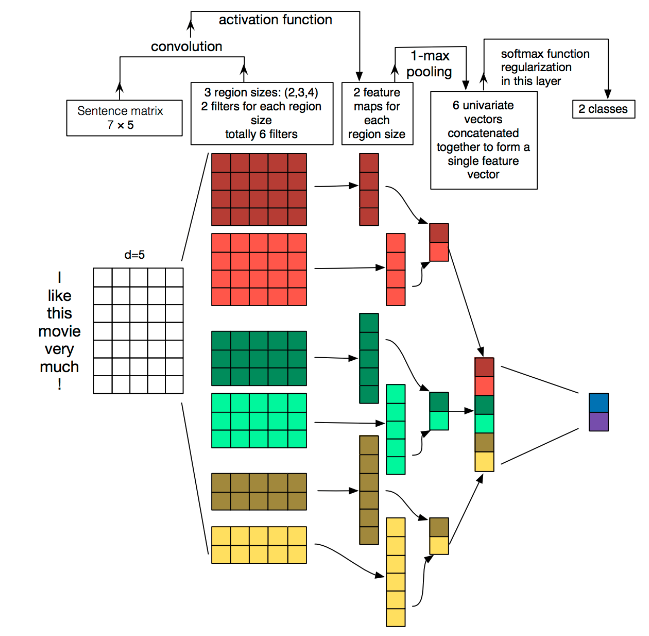
\includegraphics[width=1.\textwidth]{fig/TextCNN.png}
		\caption{TextCNN模型结构}
		\label{fig:TextCNN}
	\end{figure}
	
	输入层使用一个词向量矩阵将文本转化为词向量表示。这个词向量矩阵可以使用预训练的词向量,也可以在模型训练的过程中随机初始化。接下来,TextCNN使用多个卷积核(filter)对文本进行卷积操作,得到不同n-gram级别的特征。这里的n-gram指的是文本中连续n个词组成的片段,例如"good movie"是2-gram,"very good movie"是3-gram。每个卷积核得到的特征向量的长度取决于卷积核大小和词向量维度。在NLP任务中,卷积核大小会覆盖到词向量维度,也就是形状为[自定义长度 x 词向量维度]的矩阵,使用多个卷积核的目的是为了捕捉不同长度的n-gram特征。一般来说,TextCNN会使用多个不同大小的卷积核来分别对矩阵进行卷积,将各个卷积结果进行池化之后,拼接起来作为最终句子的特征。
	
	接下来,TextCNN通过对得到的特征向量进行最大池化操作(Max Pooling),将每个特征向量的最大值提取出来作为该特征的表示。最大池化操作的目的是为了保留特征向量中最重要的信息,丢弃无关的信息。最后,将所有池化后的特征向量拼接在一起,并通过一个全连接层输出最终的分类结果。
	
	TextCNN的优点在于它能够自动提取文本中的特征,无需手动选择特征。另外,TextCNN的计算速度比较快,因为卷积操作可以通过并行计算实现。
	
	\section{词嵌入}
	
	词嵌入是自然语言处理中的一个重要概念,它的目的是将单词映射到一个实数向量空间中,并在向量空间中捕捉到单词的语义信息。在文本分类、情感分析、机器翻译、实体识别等任务中,词嵌入是模型的重要组成部分。
	
	在传统的自然语言处理模型中,单词通常被表示为离散的整数标识。这种表示方式的问题在于无法捕捉单词之间的语义相似性。例如,将“cat”和“dog”表示为0和1,无法捕捉到它们之间的相似性,因为这两个整数之间没有数学意义上的距离或相似性。为了解决这个问题,词嵌入被引入。
	
	词嵌入的核心思想是将每个单词映射到一个向量空间中,使得向量之间的距离可以捕捉到单词之间的相似性。通常采用的方法是利用神经网络,通过学习从语料库中提取的上下文信息来学习每个单词的向量表示。
	
	一个常用的词嵌入方法是Word2Vec,它有两种模型:连续词袋模型(CBOW)和Skip-Gram模型。CBOW模型是根据周围单词的上下文来预测中心单词,而Skip-Gram模型则是根据中心单词来预测周围单词。这两种模型都通过学习单词共现的概率分布来训练词向量,并且利用了负采样或层级Softmax等技术来加速训练。
	
	另外,还有一种基于矩阵分解的词嵌入方法,即GloVe。它通过建立一个共现矩阵,然后通过SVD(奇异值分解)将该矩阵分解为两个矩阵的乘积,其中一个矩阵表示每个单词的向量表示,另一个矩阵表示单词之间的共现概率。GloVe的方法优于Word2Vec的原因在于它不仅考虑了局部上下文信息,还考虑了全局信息,因此在一些任务中表现更好。
	
	另外实践中十分常用的方式是PyTorch深度学习框架实现的nn.Embedding方法。PyTorch的nn.Embedding是一个用于实现词嵌入的神经网络层。它将离散化的词语映射到一个连续的向量空间中,从而使得机器学习模型能够更好地处理文本数据。这里的“离散化的词语”指的是以整数形式表示的词语,每个整数对应词表中的一个词。nn.Embedding将每个整数对应的词语表示成一个固定长度的向量。
	
	nn.Embedding的实现过程通常是,首先,需要为词表中的每个词语随机初始化一个固定大小的向量。然后,在前向传递过程中,将输入的整数序列作为索引传递给nn.Embedding层,它将返回一个张量,其中每行都是输入整数序列中对应词语的词向量。这些词向量在模型的训练过程中被优化,以便使它们能够更好地表示相似的词语之间的语义关系。
	
	
	\section{交叉熵损失函数}
	交叉熵损失函数(Cross-entropy loss function)是一种常用的深度学习模型的损失函数,通常用于分类问题中。其主要思想是利用目标标签和模型的预测标签之间的差距来度量模型预测的准确性,并且在训练过程中通过优化损失函数来调整模型参数,从而提高模型的预测准确性。
	
	交叉熵损失函数的定义是基于信息论中的交叉熵概念。在分类问题中,交叉熵损失函数可以表示为:
	
	$$J=-\frac{1}{N}\sum_{i=1}^{N}\sum_{k=1}^{K}y_{ik}\log{\hat{y}_{ik}}$$
	
	其中,$N$表示样本数量,$K$表示类别数量,$y_{ik}$是第$i$个样本的第$k$个标签值(0或1),$\hat{y}_{ik}$是第$i$个样本在第$k$个类别上的预测概率值。在训练过程中,我们将真实标签值表示为一个one-hot向量,即只有正确标签所在的位置为1,其他位置为0。
	
	交叉熵损失函数的本质是利用了信息熵的概念来度量模型预测的不确定性和目标标签的真实信息量之间的距离。具体来说,当模型预测正确时,交叉熵损失函数值趋近于0;当模型预测错误时,交叉熵损失函数值趋近于无穷大。因此,在训练过程中,我们通过不断调整模型参数来最小化交叉熵损失函数,从而提高模型的预测准确性。
	
	交叉熵损失函数是深度学习中常用的一种损失函数,主要用于分类问题中。其本质是基于信息论的交叉熵概念,通过度量模型预测的准确性来调整模型参数,从而提高模型的预测准确性。
	
	\section{Adam优化函数}
	Adam(Adaptive Moment Estimation)是一种基于梯度的优化算法,由\\Diederik P. Kingma和Jimmy Lei Ba于2015年提出,已成为深度学习中最常用的优化算法之一。Adam算法结合了自适应梯度方法和动量方法的优点,同时也解决了它们各自的缺点。在许多深度学习任务中,Adam比传统的随机梯度下降(SGD)和其他优化器更快、更稳定。
	
	Adam算法的核心思想是自适应性和动量。自适应性是指Adam能够自适应地调整每个参数的学习率,从而在不同的参数上使用不同的学习率。动量是指Adam将每个参数的上一步梯度考虑在内,从而增加了对先前梯度的记忆,以更好地估计当前梯度。Adam算法使用指数移动平均数来计算自适应的学习率和动量。它可以看作是RMSProp和动量优化器的结合,但是更具有鲁棒性。
	
	Adam算法的核心公式如下:
	
	$$
	m_t=\beta_1m_{t-1}+(1-\beta_1)g_t 
	$$
	$$
	v_t=\beta_2v_{t-1}+(1-\beta_2)g_t^2
	$$
	$$
	\hat{m_t}=\frac{m_t}{1-\beta_1^t}
	$$
	$$
	\hat{v_t}=\frac{v_t}{1-\beta_2^t}
	$$
	$$
	\Delta\theta_t=-\frac{\eta}{\sqrt{\hat{v_t}+\epsilon}}\hat{m_t}
	$$

	
	其中,$m_t$和$v_t$分别表示每个参数的一阶矩估计和二阶矩估计,$g_t$是当前的梯度,$\beta_1$和$\beta_2$是指数衰减率,$\hat{m_t}$和$\hat{v_t}$是对$m_t$和$v_t$的偏差修正,$\eta$是学习率,$\epsilon$是一个小常数,用于数值稳定性。
	
	Adam算法可以看作是RMSProp和动量优化器的结合。与RMSProp相似,Adam通过估计二阶矩来计算自适应学习率,但是它使用了动量来增加对先前梯度的记忆,以更好地估计当前梯度。相比于传统的SGD,Adam在不同的深度学习任务中通常能够得到更快、更稳定的收敛。
	
	
	\chapter{实验过程}
	\section{实验环境配置}
	
	本地验证环境
	\begin{table}[htbp]
		\caption{本地实验环境}
		\centering
		\renewcommand{\arraystretch}{1.5}
		\begin{tabular}{|c|ccc|}
			\hline
			操作系统                       & \multicolumn{1}{c|}{Windows11 专业版}                    & \multicolumn{1}{c|}{硬件环境}                 & CUDA 11.1            \\ \hline
			深度学习框架                     & \multicolumn{1}{c|}{PyTorch 1.10.1+cu113}             & \multicolumn{1}{c|}{Python版本}             & 3.8.10               \\ \hline
			\multicolumn{1}{|l|}{运行说明} & \multicolumn{3}{l|}{\begin{tabular}[c]{@{}l@{}}1. 首先运行Exp3\_DataProc.py文件,构建词表并保存至本地磁盘。\\
			2. 运行Exp3\_Main.py文件,此时会首先检查此前是否已经训练并\\保存过checkpoint文件,若保存过则继续训练,否则从头开始训练,\\程序会将验证集上表现最好的模型进行保存。并在训练结束后对测\\试集推理。\\
			3. 如需修改全局配置参数,可进入Exp3\_Config.py文件修改。
			\end{tabular}} \\ \hline
		\end{tabular}
	\end{table}
		

	\section{数据预处理}
	实验需要对数据进行一定的预处理,在Exp3\_DataProc.py文件中共实现了两个类,功能分别为处理句子和实现将标签和与之对应的ID相互转换。具体来说,分别实现了两个类:SentenceProcess 和 RelationAndID 。
	
	SentenceProcess类中,主要的方法和功能如下:
	
	\begin{enumerate}
		\item \textbf{build\_vocab 方法}\quad 这个方法用于构建词典(vocabulary)。传入的参数是 filepath 和 vocab\_size,分别表示训练集的路径和词典大小。首先,这个方法会读取训练集,计算出其中每个单词的出现次数,然后根据出现次数排序,取出出现次数最多的 vocabsize 个单词作为词典。使用torchtext库中封装的 build\_vocab\_from\_iterator 方法将 counter\_sorted 转换为 Vocab 对象。接着,将词典中的 token 映射到索引,并保存到文件中。
		
		\item \textbf{sentence2index方法} \quad 这个方法用于将一个句子转换为索引。传入的参数是一个词典和一个句子。方法首先遍历句子中的每个单词,查找它在词典中的索引。如果单词不在词典中,就随机生成一个索引,并将它添加到 sentence\_id 列表中。最后返回 sentence\_id 列表。
		
		\item \textbf{index\_sentence\_position\_mask方法} \quad 该方法是此类中比较重要的方法,它将一个输入的文本数据(原始数据 original\_data 中)转换为模型可用的输入格式,即将文本转换为对应的索引序列,并计算出每个词到实体位置的相对距离,将这些位置信息转换为相对位置索引,并进行 padding 和 mask 操作,最后将其转换为 PyTorch 张量。
		
		具体来说,这段代码的主要步骤如下:
		
		\begin{enumerate}
			\item 对原始文本进行分词,并读取预先保存的词汇表(通过 vocab\_path 指定),将分词后的句子转换为对应的索引序列(即将每个单词转换为其在词汇表中的索引),得到 sentence\_index。
			
			\item 从 original\_data 中获取 head 和 tail 两个实体,并计算出它们在文本中的位置(分别存储在 ent1pos 和 ent2pos 变量中)。
			
			\item 对于每个单词,计算其到 head 和 tail 实体位置的相对距离,并将其转换为相对位置索引,分别存储在 pos1 和 pos2 变量中。
			
			\item 对于位置序列(即 pos1 和 pos2),如果长度不足 max\_sentence\_length,则进行 padding 操作,即在序列末尾加入 0 直至长度达到 max\_sentence\\\_length。然后,将序列截断至 max\_sentence\_length 长度。
			
			\item 对于文本中每个单词,根据其在文本中的位置,将其分为三类(在实体1之前,实体1和实体2之间,和实体2之后),并将其转换为对应的 mask 序列,分别存储在 mask 变量中。
			
			\item 对于 mask 序列,如果长度不足max\_sentence\_length,则进行 padding 操作,即在序列末尾加入 0 直至长度达到 max\_sentence\_length。然后,将序列截断至 max\_sentence\_length 长度。
			
			\item 对于 sentence\_index, pos1, pos2 和 mask 四个序列,将其转换为 PyTorch 张量,并以列表的形式返回。
		\end{enumerate}
		
		\item \textbf{get\_position方法} \quad 获取一个单词在句子中的位置信息.将单词在句子中的位置信息转换为一个正整数,这个正整数的范围是从 0 到 $pos\_limit \times 2 + 1$。
	\end{enumerate}
	
	RelationAndID类则较为简单,通过读取存储标签-ID的json文件,实现标签和ID的呼唤,代码编写如图\ref{fig:rai}所示。
	
	\begin{figure}[htbp]
		\centering
		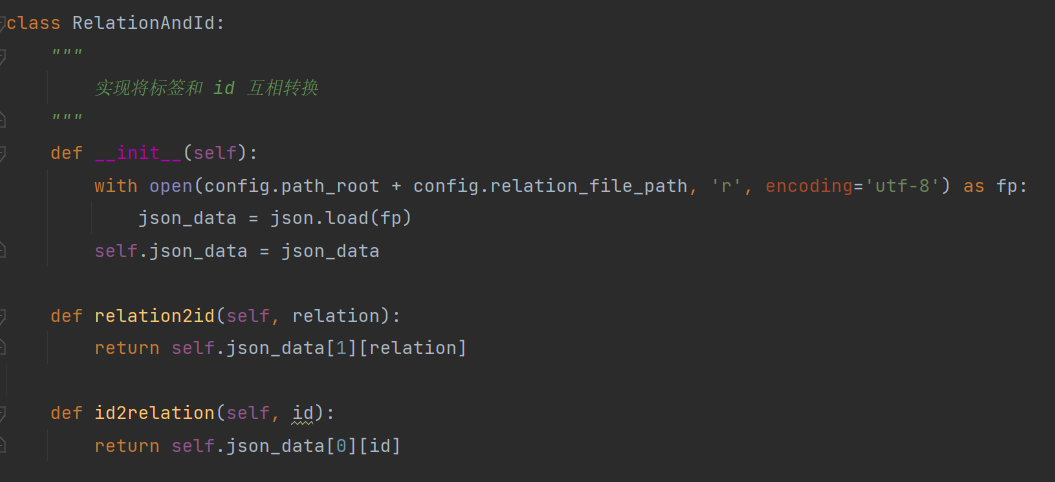
\includegraphics[width=1.\textwidth]{fig/rai.png}
		\caption{标签与ID转换}
		\label{fig:rai}
	\end{figure}
	
	\section{自定义数据加载器}
	实验的数据集是中文医学数据,共三万多条训练数据。由于训练集和验证集与测试集的数据有所不同,故分别实现两个略有不同的类。具体来说,训练集和验证集中的数据包括有头实体、尾实体、关系(标签)和文本,测试集中则不包含关系(标签)。数据的示例结构如图\ref{fig:train}与图\ref{fig:test}所示。
	
	\begin{figure}[htbp]
		\centering
		\begin{minipage}[t]{1.0\textwidth}
			\centering
			\centering
			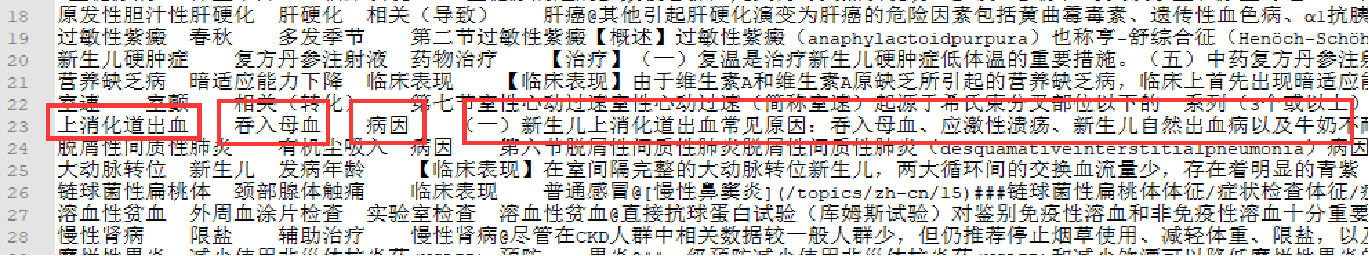
\includegraphics[width=1.0\textwidth]{fig/traindata.png}
			\caption{训练集与验证集}
			\label{fig:train}
		\end{minipage}
		
		\begin{minipage}[t]{1.0\textwidth}
			\centering
			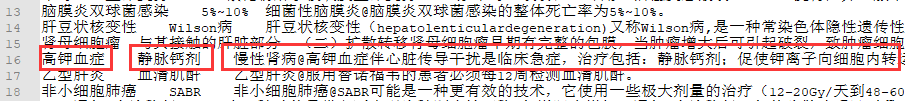
\includegraphics[width=1.0\textwidth]{fig/testdata.png}
			\caption{测试集}
			\label{fig:test}
		\end{minipage}
	\end{figure}
	
	数据集处理类通过继承PyTorch框架里的Dataset类来实现,该类的作用是读取给定文件中的文本数据并将其转换为模型可用的格式。以训练集的处理类为例,该类的主要方法如下:
	\begin{enumerate}
		\item \_\_init\_\_ 方法:读取文件路径对应的文本数据,并按照一定的格式进行处理。具体来说,将每一行文本数据中的头部、尾部、关系和句子文本分别提取出来,组成一个字典,并将这个字典添加到 original\_data 列表中。
		
		\item \_\_getitem\_\_ 方法:根据给定的索引 index,获取 original\_data 列表中对应的一个文本数据,并调用 SentenceProcess 类中的方法将句子文本进行处理得到一个经过 mask 处理后的序列列表 seq,并调用 RelationAndId 类中的方法将关系名称转换成相应的标签 label,将二者一起返回。
		\item \_\_len\_\_ 方法:返回 original\_data 列表的长度,即表示该数据集一共包含多少个文本数据。
	\end{enumerate}
	
	
	\section{模型定义}
	本实验实现了一个用于关系抽取的TextCNN模型。这个神经网络继承自PyTorch中的nn.Module类,用于封装神经网络的结构和前向传播函数。
	
	在网络的初始化函数\_\_init\_\_()中,定义了该模型需要用到的超参数,包括一些卷积操作的参数,如卷积核的大小、填充的大小等,以及模型需要输出的标签数目。
	
	该模型的结构包括三个嵌入层:词嵌入、实体位置嵌入1、实体位置嵌入2;一个卷积层conv;一个dropout层;一个池化层pool;一个全连接层out\_linear。
	
	在前向传播方法forward中,将输入数据data中的四个tensor(token、pos1、pos2、mask)在嵌入层中进行嵌入操作,并将三个嵌入层的输出拼接在一起得到一个shape为(B, L, EMBED)的张量x。通过卷积层conv,将x转换为(B, H, L)的张量。通过mask\_embedding将mask映射到3维空间,并用1减去这个张量得到一个(B, L, 3)的mask张量,用它对卷积层的输出x进行掩码操作(即将mask对应位置的值替换为一个非常小的负数),并在掩码后的结果上分别通过池化层得到3个(B, H, 1)的池化张量,将它们拼接在一起得到一个(B, 3H, 1)的张量。然后对这个张量进行一些操作,包括对第二个维度进行squeeze操作(将第二个维度压缩为1),dropout层的操作以及全连接层的操作,得到最终的输出张量x。
	
	图\ref{fig:ckpt}为保存后的模型结构。
	
	\begin{figure}[htbp]
		\centering
		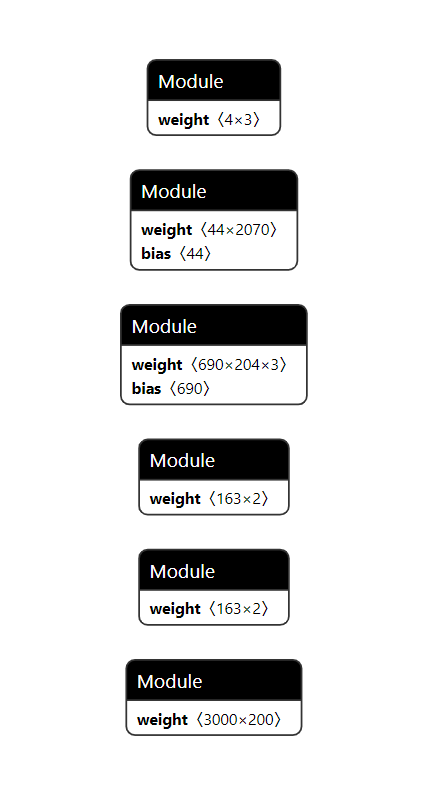
\includegraphics[width=0.4\textwidth]{fig/ckpt.png}
		\caption{保存的checkpoint模型}
		\label{fig:ckpt}
	\end{figure}
	
	
	\chapter{实验结果与分析}
	\section{结果}
	实验运行结果如截图\ref{fig:run}所示。
	
	\begin{figure}[!htbp]
		\centering
		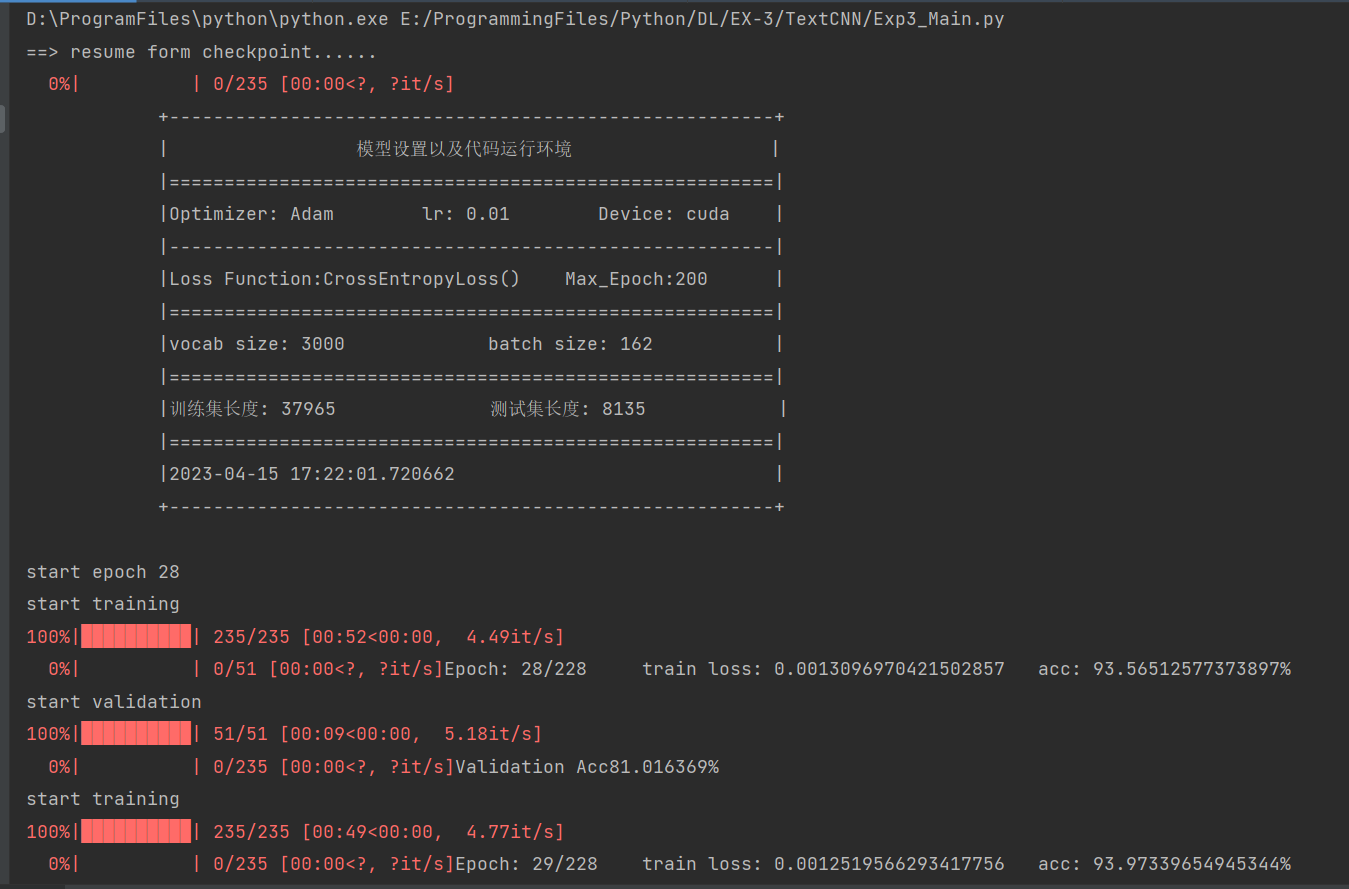
\includegraphics[width=1.2\textwidth]{fig/running.png}
		\caption{模型训练过程}
		\label{fig:run}
	\end{figure}

	实验开始设置了100次epoch,运行中观察到在迭代到15次左右时验证集的增长速度十分缓慢,到40次左右时准确率出现了下降的趋势,推测此时出现了过拟合的现象。在提交的代码中,迭代次数调整至64次,验证时保存验证准确率最高的模型,利用测试集推理时加载保存的最佳模型。
	
	\section{出现的问题及分析}
	
	\begin{enumerate}
		\item 读取数据,对应头实体与尾实体的相对位置信息时,出现报错信息,显示在文本中找不到实体。检查发现部分数据中头实体或尾实体缺失或不存在头尾实体,而是采用了占位符。针对这种情况,将头实体的位置指定位0,尾实体指定为-1。
		
		\item 验证集上最佳的的准确率只能达到81.64\%。推测这是模型本身的缺点所导致的。缺乏上下文信息。TextCNN 没有显式地考虑单词之间的上下文信息,因此在需要考虑上下文信息的 NLP 任务中可能表现不佳。此外,卷积操作可能损失一些信息。由于卷积操作是一种局部操作,可能会损失一些全局的语义信息,这也是 TextCNN 的一个局限。
	\end{enumerate}
	
	
	\chapter{心得 体会}
	首先,针对数据处理方面,本实验使用的数据集是一个实体关系抽取的数据集,对数据集进行预处理是一个比较大的挑战,包括读取数据集,进行分词处理等。在这个实验中,使用了Pytorch框架中提供的nn.Embedding\\来进行词嵌入的操作,其目的是将原始的词汇映射为向量空间中的稠密向量,从而使得相似的词汇在向量空间中距离更近。另外,还使用了Max-Pooling和Dropout等技术,以防止模型过拟合和提高模型的泛化能力。
	
	其次,针对模型搭建方面,本实验使用了TextCNN模型来进行实体关系抽取。该模型包含词嵌入层、卷积层、最大池化层、Dropout层和全连接层等部分。其中,词嵌入层用来将输入的词汇转化为向量表示,卷积层用来提取句子的局部特征,最大池化层用来减小特征向量的维度,Dropout层用来防止模型过拟合,全连接层用来输出模型的预测结果。此外,模型还使用了一些超参数,如filter\_num、word\_dim、pos\_dim、kernel\_size、padding\_size\\等,这些超参数都需要根据实际数据集的情况进行调整。
	
	由于时间与个人能力等方面的原因,实验中对网络资源的依赖比较大,且最终的实验结果只能达到81\%左右,实验效果有所欠缺。但是本实验采用TextCNN模型对实体关系抽取任务进行了探究,通过数据处理、词嵌入、分词、模型搭建等步骤进行了详细的学习、分析和实验,为实现能力提升提供了一定的裨益,实验题目本身也是很好的学习材料。
	
	
\end{document}





